\chapter{Аргачлал ба загварчлал}
Энэ бүлгийн 3.1-т системийн ерөнхий бүтцийг, 3.2-т загвар сонголтын туршилт ба үр дүнг, 3.3--3.7-д хэрэгжүүлсэн хүн хуваарилалт, урьдчилсан боловсруулалт, синхрончлолын алгоритм болон хэрэгжүүлэлтийн орчныг тайлбарлав.

\section{Системийн ерөнхий бүтэц}

Систем нь хоёр болон түүнээс дээш хүний хөдөлгөөнийг агуулсан видео бичлэгийг оролт болгон авч, синхрончлолын оноо болон түүнийг тайлбарлах графикуудыг гаралт болгон гаргана. Боловсруулалт дараах дарааллаар явагдана.

\begin{enumerate}
\def\labelenumi{\arabic{enumi}.}
\item
  \textbf{Оролт:} Олон хүний хөдөлгөөнийг агуулсан видео бичлэгийг кадр бүрээр уншина.
\item
  \textbf{Гол цэг илрүүлэлт:} Сонгосон HPE загвараар кадр бүрээс хүн тус бүрийн гол цэгүүдийн координат болон итгэлцлийн оноог гаргана. Энэ алхмыг хэрэглэгчийн вэб хөтөч дээр эсвэл сервер дээр гүйцэтгэж болно (3.7).
\item
  \textbf{Хүн хуваарилалт:} Илэрсэн араг ясуудыг зүүнээс баруун тийш 1, 2, ..., N дугаартай хүнд тогтмол хуваарилж, хүн бүрт хугацааны цуваа үүсгэнэ.
\item
  \textbf{Урьдчилсан боловсруулалт:} Итгэлцэл багатай цэгүүдийг нөхөх, шуугианыг тэгшитгэх үйлдлийг гүйцэтгэнэ.
\item
  \textbf{Шинж чанар гаргах:} Гол цэгүүдээс үений өнцгүүдийг тооцоолно.
\item
  \textbf{Синхрончлолын тооцоолол:} Хүмүүсийн хос бүрт орон зайн болон хугацааны хэмжүүрүүдийг тооцоолж, хосуудын онооны дунджаар бүлгийн нэгдсэн оноо гаргана.
\item
  \textbf{Синхрончлол алдагдсан мөчүүд:} Хос бүрт синхрончлол алдагдсан хугацааны хэсэг, хоцорсон хүн болон биеийн хэсгийг илрүүлнэ.
\item
  \textbf{Үр дүнг харуулах:} Боловсруулалтын явцад араг яс зурагдсан видеог үүсгэж, дараа нь тэр видеог тоглуулахдаа тухайн мөчийн синхрончлолын оноо, биеийн хэсэг бүрийн оноо, цагийн хоцрогдлыг хажууд нь бодит хугацаанд харуулна.
\end{enumerate}

\section{Загвар сонголт}

Загвар сонгохдоо дараах шалгуурыг баримтална. Үүнд: даалгаварт шаардлагатай гол цэгийн тоо, нэг кадрт олон хүнийг нэгэн зэрэг илрүүлэх чадвар, гол цэг илрүүлэлтийн нарийвчлал, боловсруулалтын хурд, ашиглахад хялбар байдал.

Эдгээр шалгуурын дагуу таван загварыг нэг ижил видео бичлэг дээр ажиллуулж харьцуулав. Харьцуулалтад YOLOv8n, YOLO11n (нэг алхамт), RTMPose-m, ViTPose-B (дээрээс доош, ижил хүн илрүүлэгчтэй) болон MediaPipe Pose загваруудыг хамруулсан. Туршилтын бичлэг 25 кадр/с давтамжтай, ойролцоогоор 34 секунд үргэлжлэх бөгөөд гурван хүнтэй. Энэ нь системийн үндсэн тохиолдол болох хоёр хүнээс хүнд нөхцөл бөгөөд олон хүнтэй бичлэгт загваруудын ажиллагааг шалгах боломж олгоно. Таван туршилт бүгд ижил файл дээр хийгдсэнийг SHA-256 хэшээр баталгаажуулсан. Хурдыг браузер дотор хэмжсэн бөгөөд MediaPipe WebGL, бусад дөрвөн загвар WebGPU дээр ажилласан.

Туршилтын бичлэгт гурван хүн цэнхэр дэвсгэрийн өмнө зэрэгцэн зогсож, тулааны урлагийн ижил хөдөлгөөнийг хийж байгаа бөгөөд хүмүүс хэсэгчлэн давхцаж харагддаг (Зураг~\ref{fig:fig0_test_video}). Иймд энэ бичлэг нь олон хүнийг зэрэг илрүүлэх, хажуугаас харагдах байрлал болон давхцалтай нөхцөлд загваруудыг шалгахад тохиромжтой.

\begin{figure}[H]
\centering
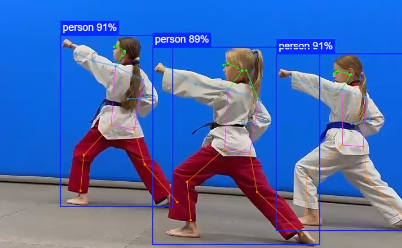
\includegraphics[width=0.75\linewidth]{fig0_test_video}
\caption{Загвар сонголтын туршилтад ашигласан бичлэгийн нэг кадр (илэрсэн хүмүүсийн хүрээ ба араг яс)}
\label{fig:fig0_test_video}
\end{figure}

Бичлэгт гол цэгүүдийн жинхэнэ байрлал (ground truth) тэмдэглэгдээгүй тул гол цэгийн чанарыг шууд бус үзүүлэлтээр үнэлэв. Үүнд: бусад дөрвөн загварын медиантай хэр нийцэж буйг харуулах тохирол (PCK@0.05, биеийн өндрийн 5\%-ийн дотор), дараалсан кадрууд хооронд гол цэг хэр чичирч буйг харуулах чичиргээ (jitter), гар, хөлийн урт бичлэгийн туршид хэр тогтвортой байгааг харуулах мөчдийн уртын хэлбэлзлийн коэффициент.

\textbf{Олон хүний илрүүлэлт.} YOLOv8n, YOLO11n, RTMPose-m, ViTPose-B загварууд кадрын 100\%-д гурван хүнийг бүгдийг нь илрүүлсэн бол MediaPipe зөвхөн 30\%-д нь илрүүлсэн (Зураг~\ref{fig:fig1_detection}). Кадр бүрт илэрсэн хүний тооны графикаас MediaPipe-ийн илрүүлэлт бичлэгийн туршид тасралтгүй хэлбэлзэж байгаа нь харагдана. Бусад загварт хааяа гурваас олон хүн илэрсэн богино хугацааны худал илрүүлэлт ажиглагдсан бөгөөд худал илрүүлэлтгүй кадрын хувь YOLOv8n-д 98.6\%, YOLO11n-д 97.8\%, RTMPose-m болон ViTPose-B-д 97.1\% байв.

\begin{figure}[H]
\centering
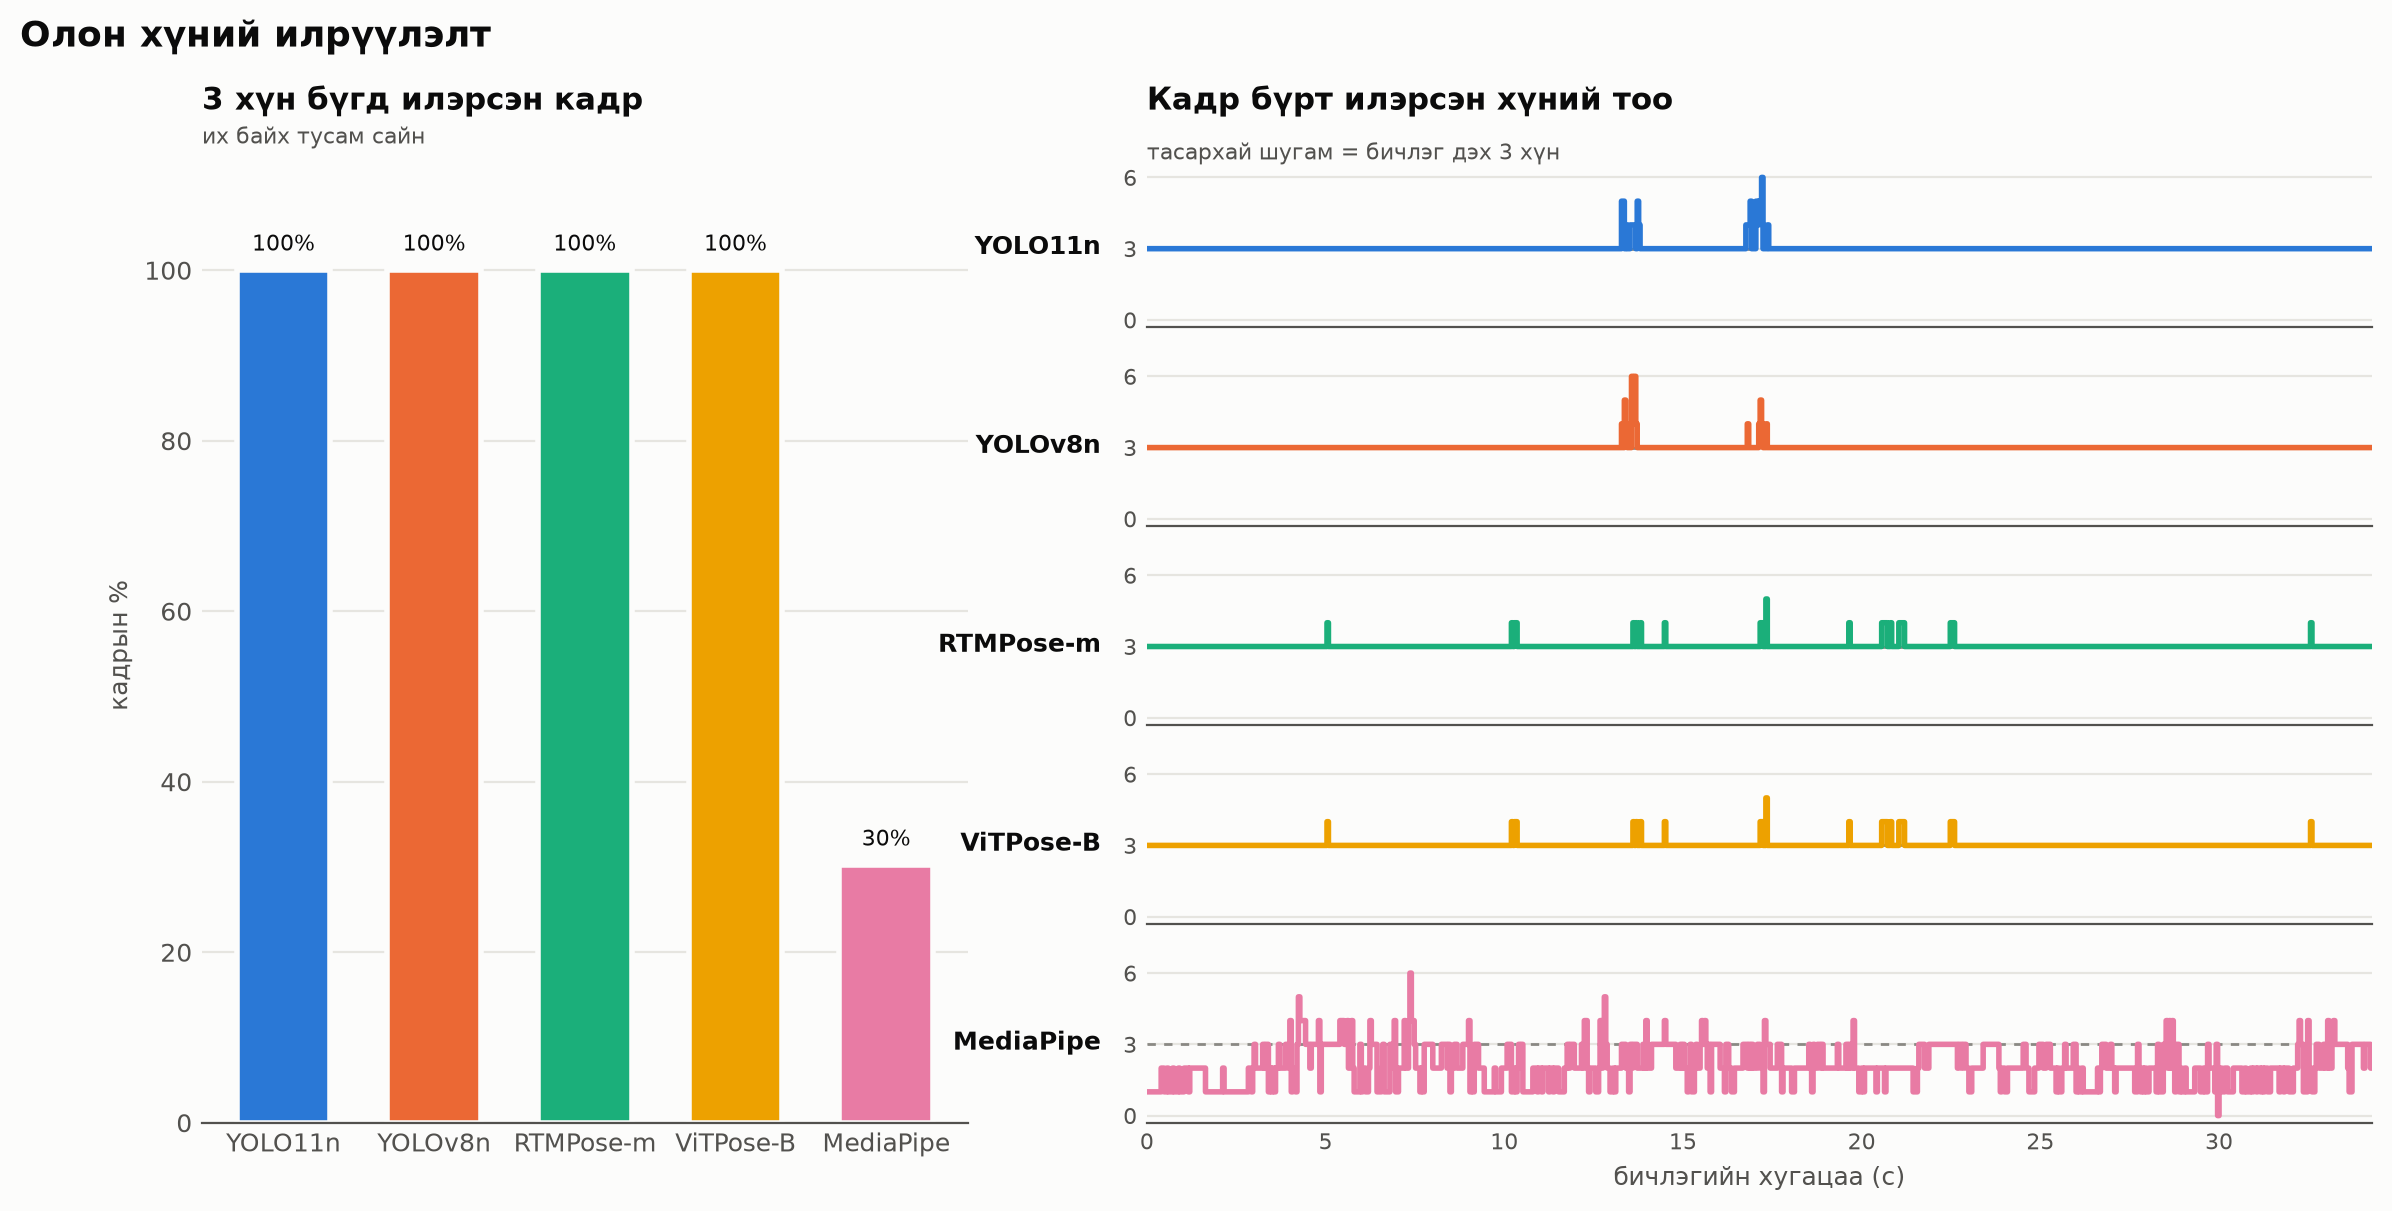
\includegraphics[width=\linewidth]{fig1_detection}
\caption{Гурван хүн бүгд илэрсэн кадрын хувь ба кадр бүрт илэрсэн хүний тоо}
\label{fig:fig1_detection}
\end{figure}

\textbf{Боловсруулалтын хурд.} Нэг кадрын дундаж хугацаа MediaPipe-д 37 мс, YOLOv8n-д 42 мс, YOLO11n-д 46 мс байсан бол RTMPose-m-д 119 мс, ViTPose-B-д 137 мс байв (Зураг~\ref{fig:fig2_speed}). Илэрсэн нэг хүнд ногдох хугацаа RTMPose-m-д 39 мс, ViTPose-B-д 45 мс байгаа нь дээрээс доош загварууд хүн бүрийг тусад нь боловсруулдаг тул хүний тоо нэмэгдэхэд удааширдгийг харуулж байна.

\begin{figure}[H]
\centering
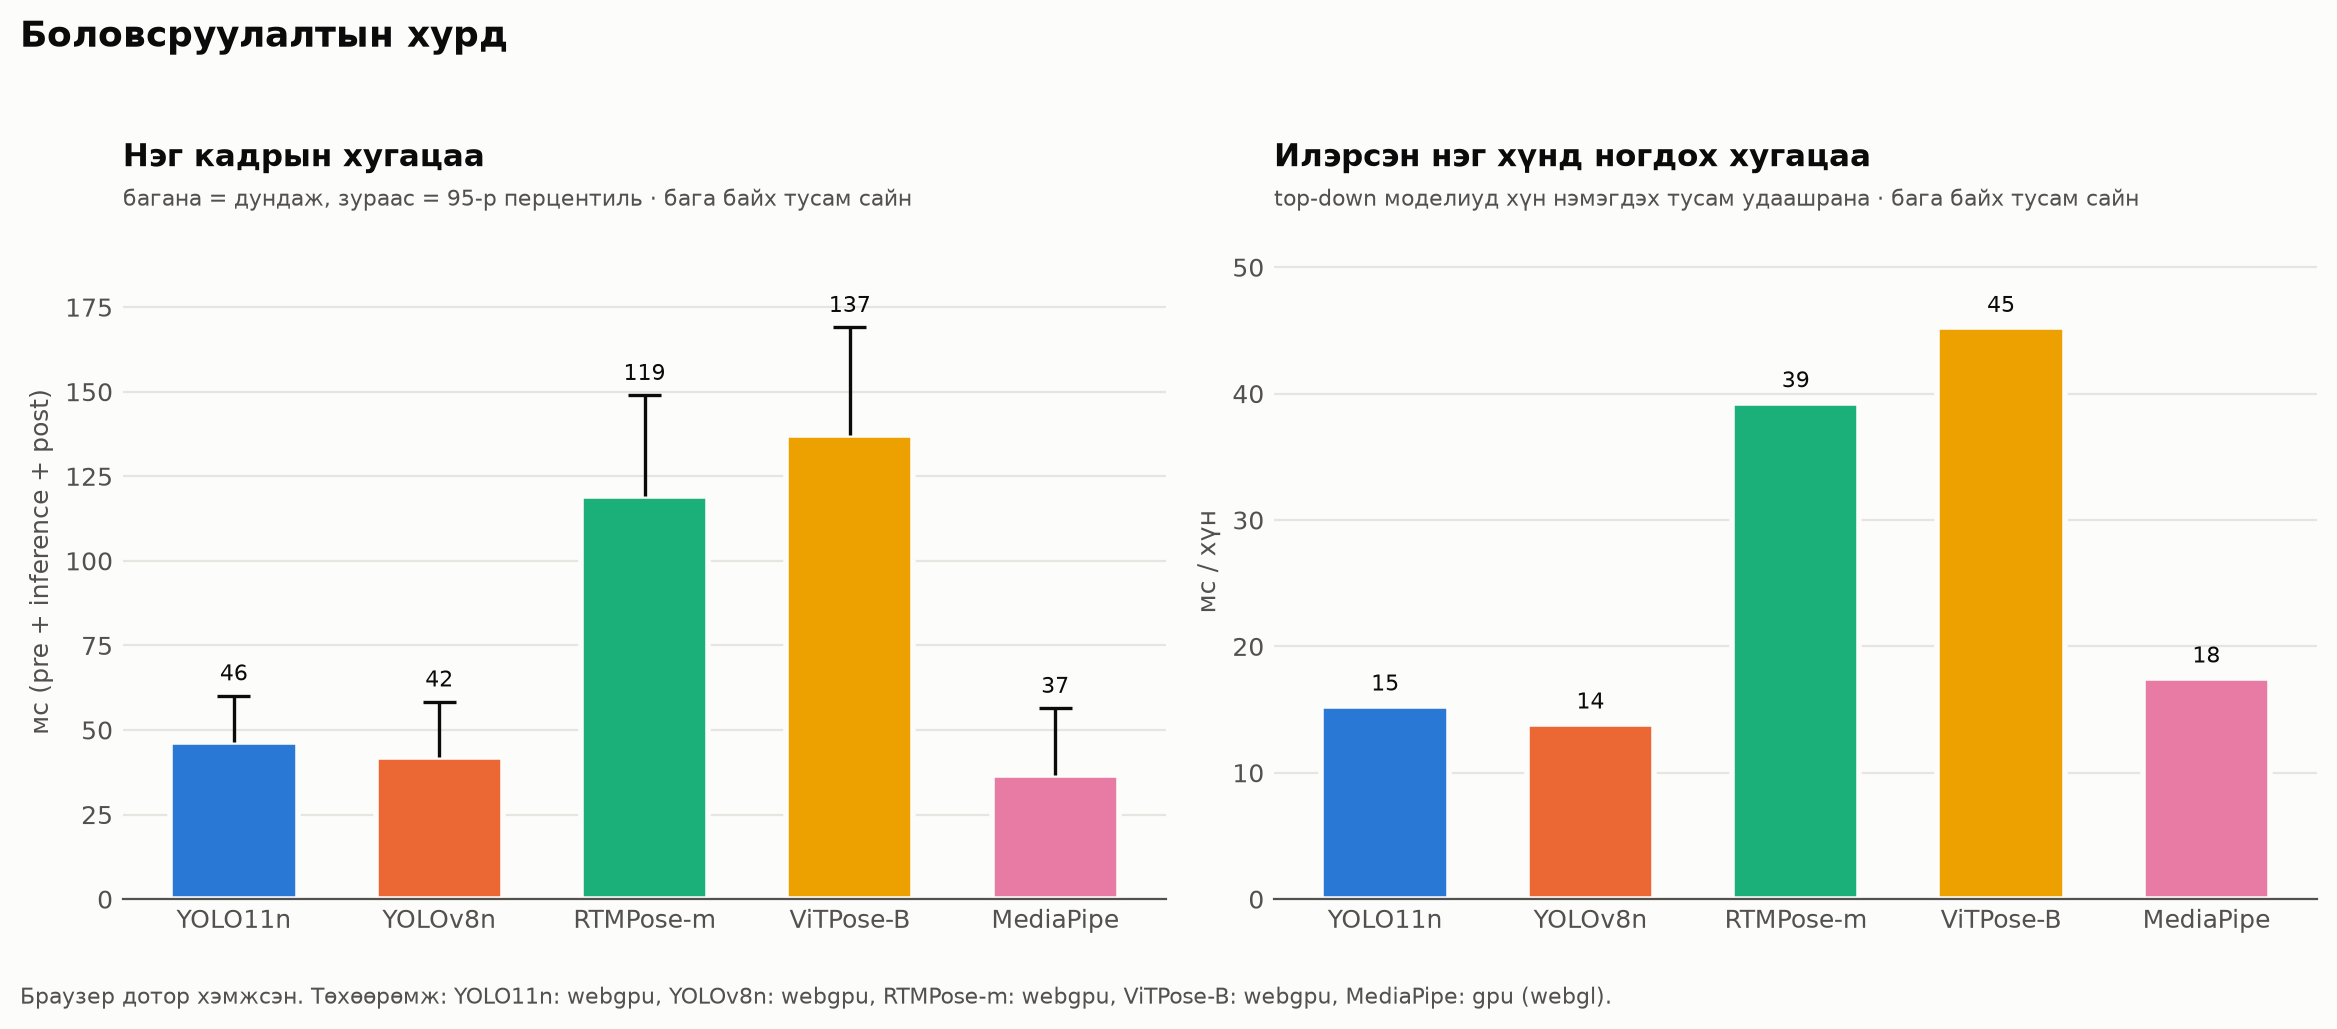
\includegraphics[width=\linewidth]{fig2_speed}
\caption{Нэг кадрын хугацаа (дундаж, 95-р перцентиль) ба илэрсэн нэг хүнд ногдох хугацаа}
\label{fig:fig2_speed}
\end{figure}

\textbf{Гол цэгийн чанар.} Тохирлын хувьд RTMPose-m (93.4\%), ViTPose-B (92.9\%), YOLOv8n (92.5\%), YOLO11n (91.3\%) хоорондоо ойролцоо байсан бол MediaPipe 71.1\%-тай байв (Зураг~\ref{fig:fig3_keypoint_quality}). Чичиргээ хамгийн бага нь RTMPose-m (1.49), хамгийн их нь MediaPipe (9.02) бөгөөд MediaPipe бусад загвараас 4-6 дахин их чичиргээтэй байв. Мөчдийн уртын тогтвортой байдлаар мөн RTMPose-m хамгийн сайн үр дүн (18.7\%) үзүүлсэн.

\begin{figure}[H]
\centering
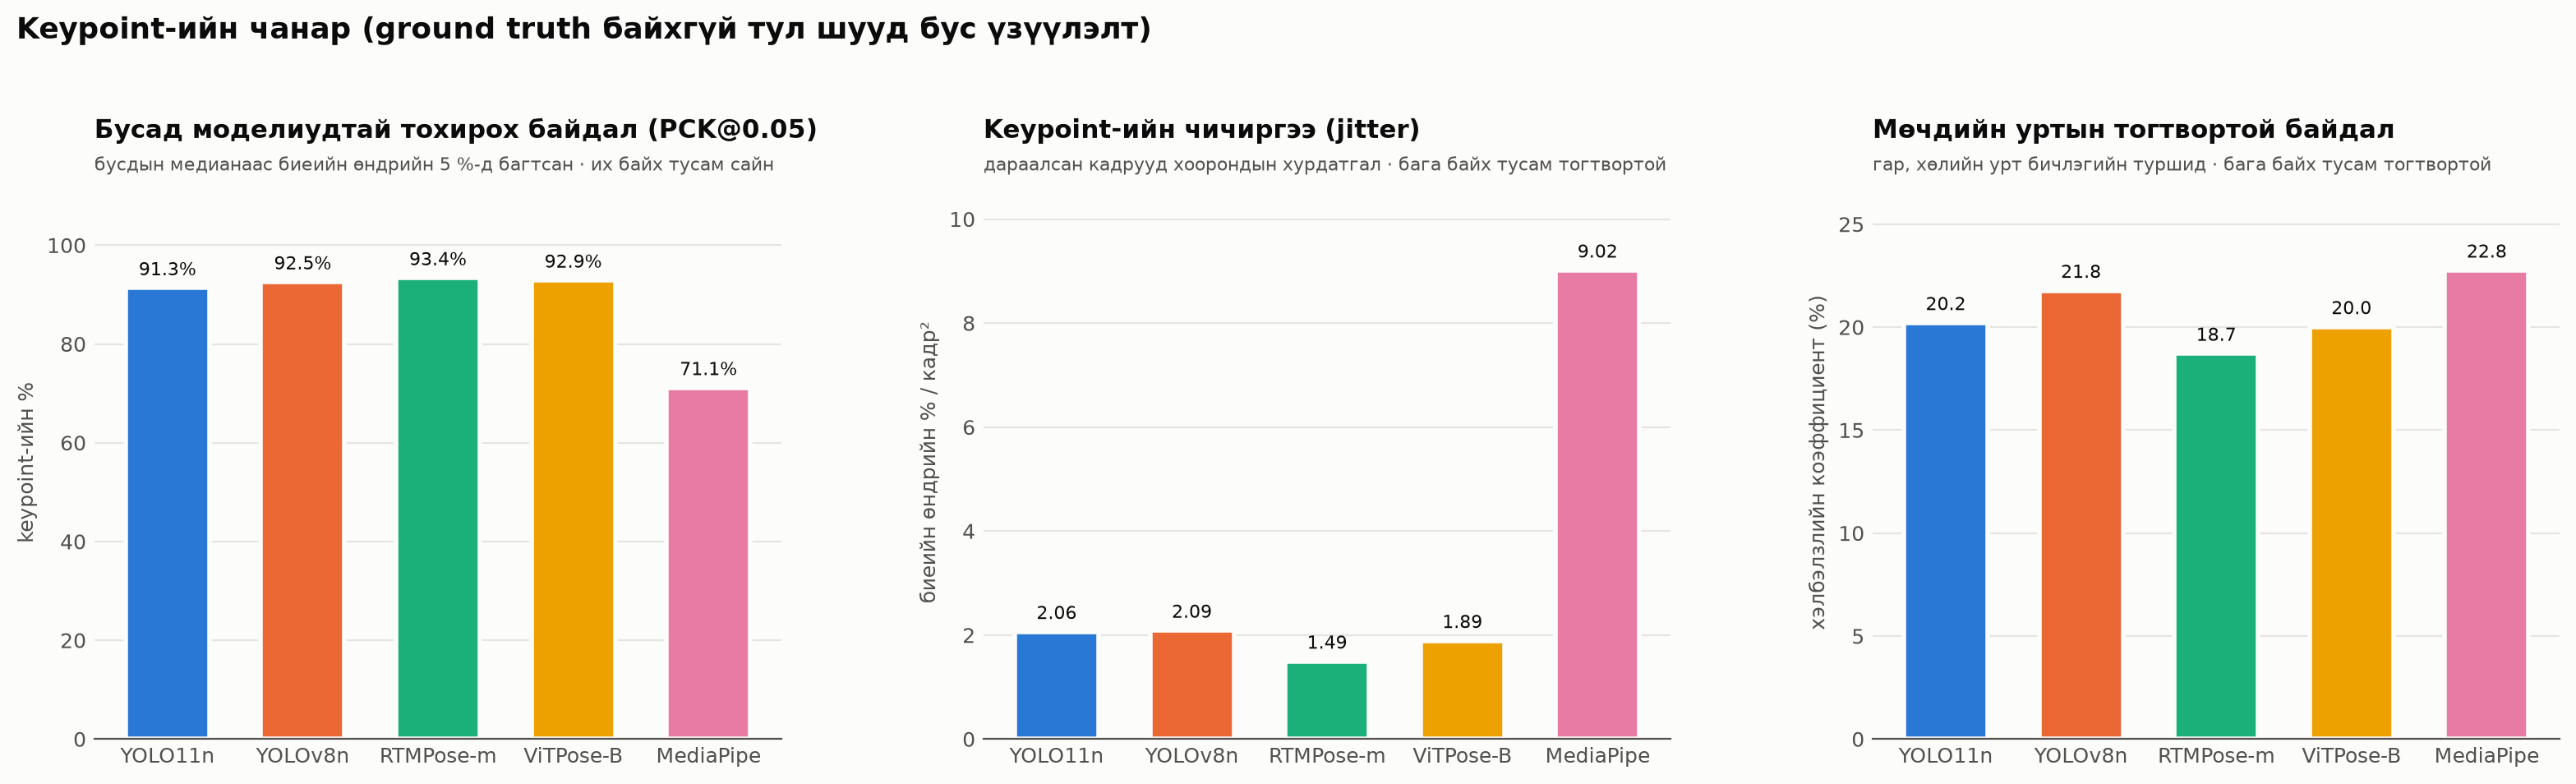
\includegraphics[width=\linewidth]{fig3_keypoint_quality}
\caption{Бусад загваруудтай тохирох байдал, чичиргээ ба мөчдийн уртын тогтвортой байдал}
\label{fig:fig3_keypoint_quality}
\end{figure}

Гол цэг тус бүрээр авч үзвэл бүх загварт бугуй, шагай, тохой, өвдөгний цэгүүд хамгийн их чичиргээтэй, нүүрний цэгүүд хамгийн тогтвортой байв (Зураг~\ref{fig:fig4_keypoint_heatmap}). Энэ нь хөдөлгөөн ихтэй, хурдан хөдөлдөг мөчдийн төгсгөлийн цэгүүдийг илрүүлэх хамгийн хэцүү байдгийг харуулна. Эдгээр цэгүүд нь 3.5-д тодорхойлсон тохой, өвдөгний өнцгийг тооцоолоход шууд ашиглагддаг тул синхрончлолын үнэлгээнд онцгой чухал. Бугуйн чичиргээ RTMPose-m-д 2.6-3.1 байхад YOLO11n-д 4.3-4.5, MediaPipe-д 12.9-13.2 байв.

\begin{figure}[H]
\centering
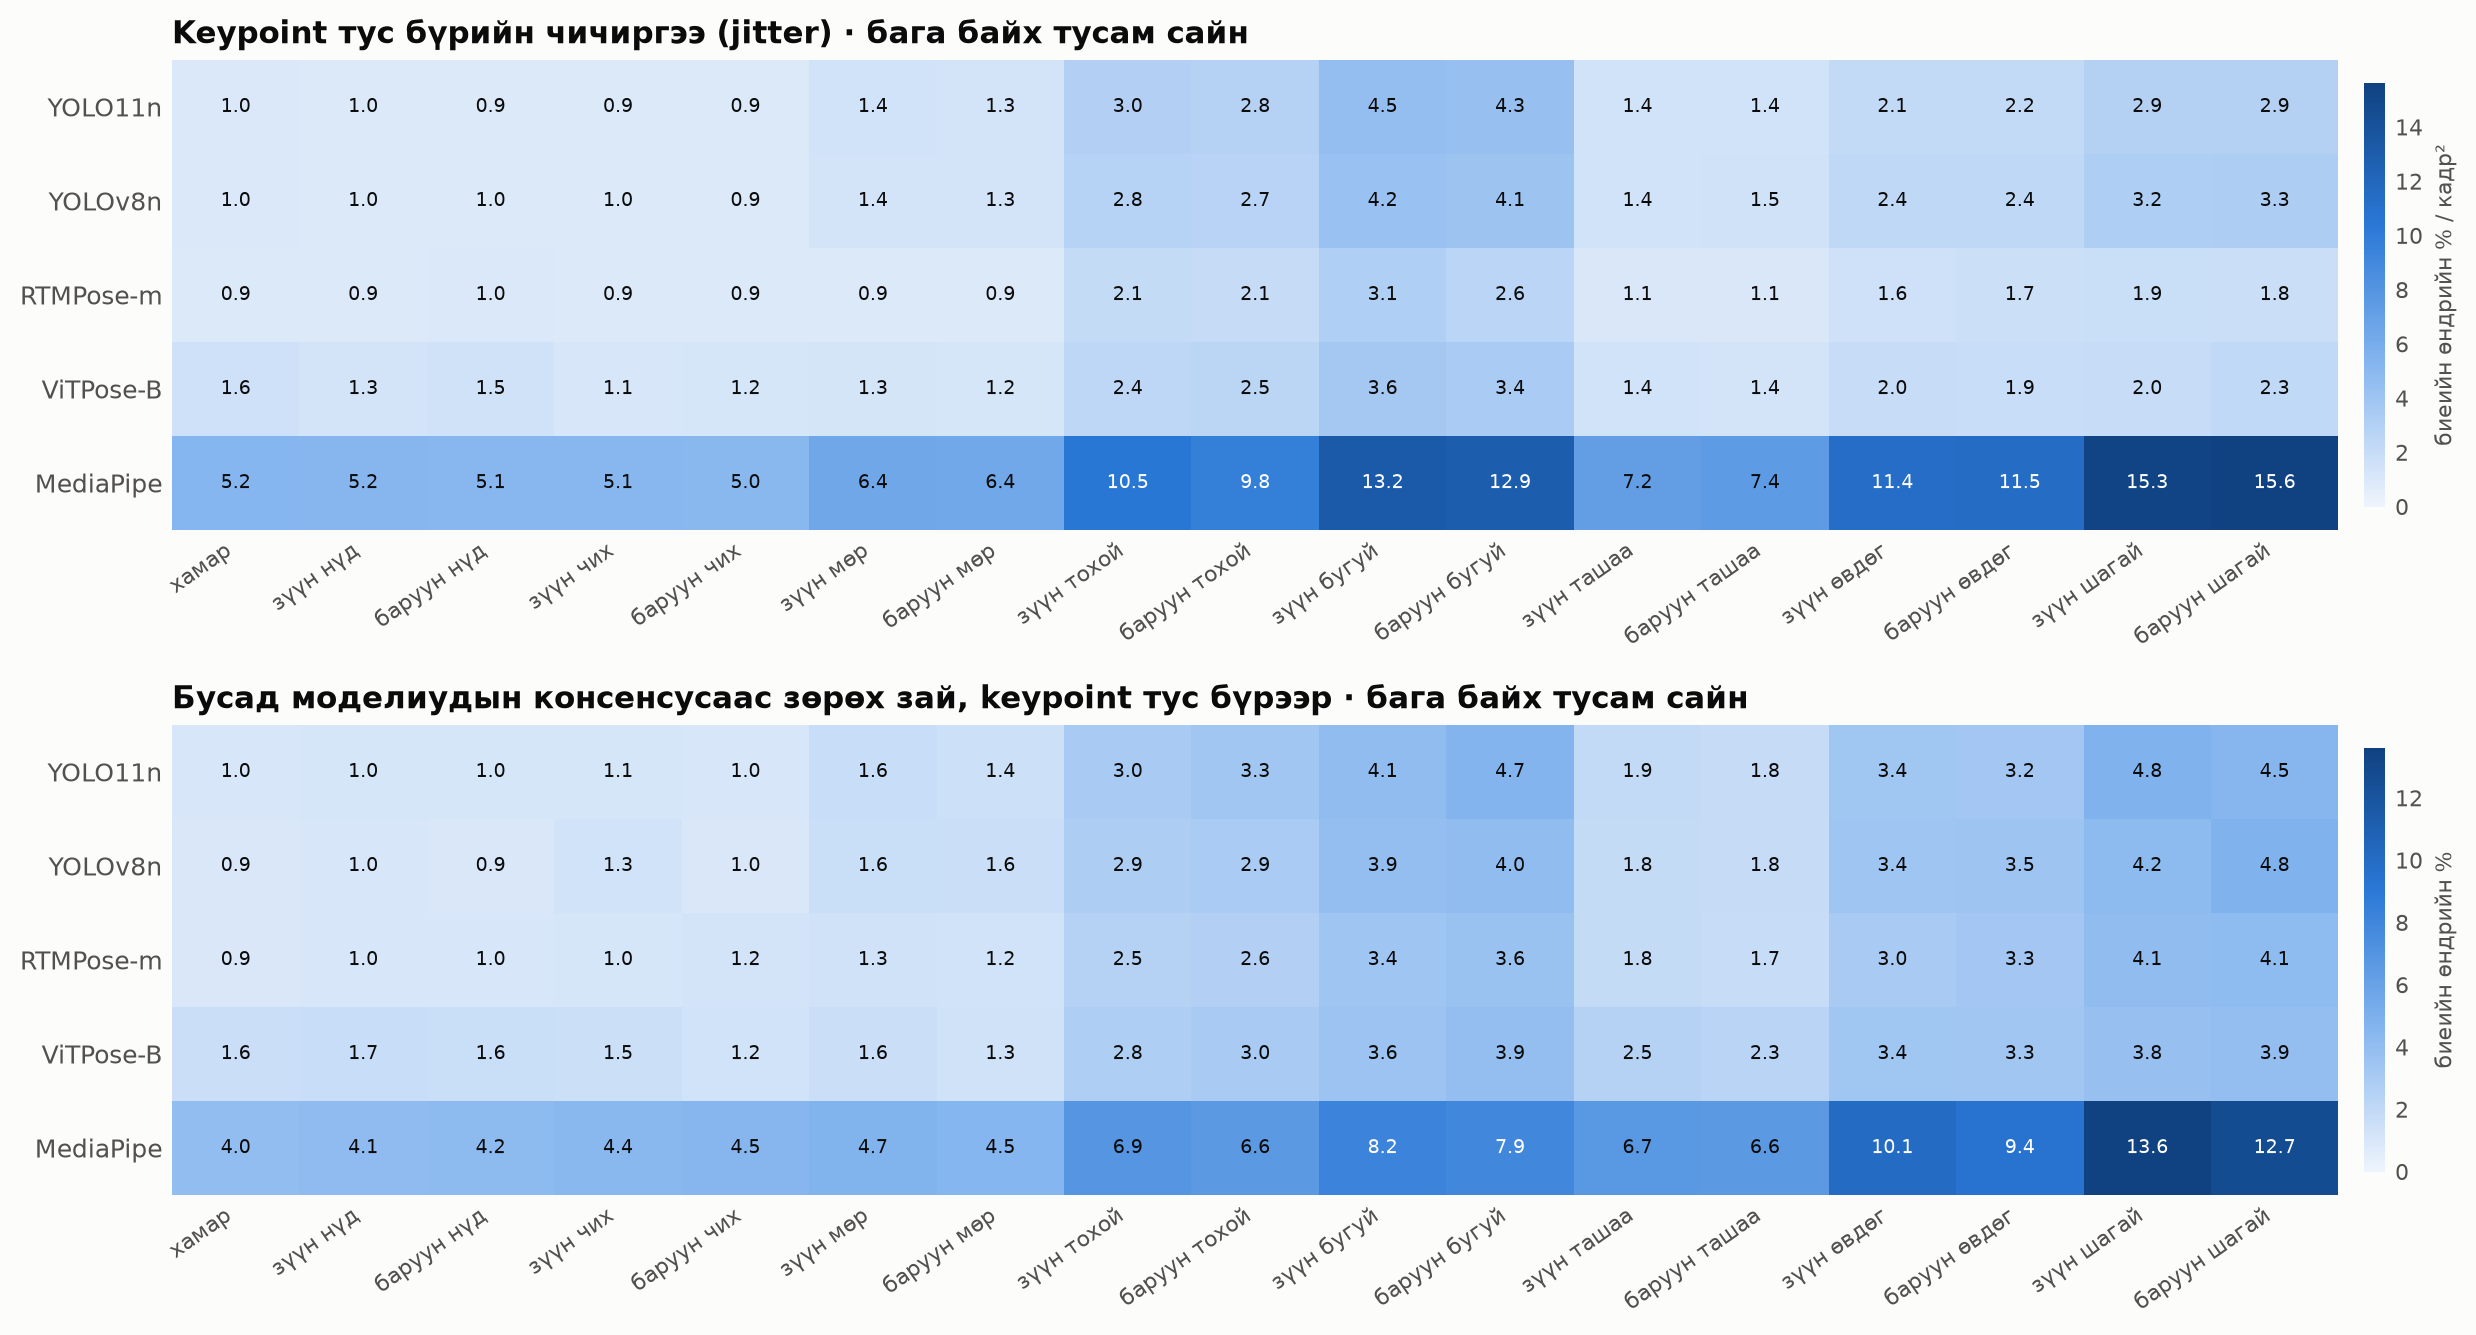
\includegraphics[width=\linewidth]{fig4_keypoint_heatmap}
\caption{Гол цэг тус бүрийн чичиргээ болон бусад загваруудын консенсусаас зөрөх зай}
\label{fig:fig4_keypoint_heatmap}
\end{figure}

\textbf{Хурд ба чанарын харьцаа.} Зураг~\ref{fig:fig5_tradeoff}-д загваруудыг хурд ба тохирлоор нь байршуулсан. YOLOv8n, YOLO11n загварууд хурдан бөгөөд тохирол өндөр, RTMPose-m, ViTPose-B загварууд тохирол бага зэрэг илүү боловч ойролцоогоор гурав дахин удаан, харин MediaPipe хурдан боловч тохирол мэдэгдэхүйц бага байна.

\begin{figure}[H]
\centering
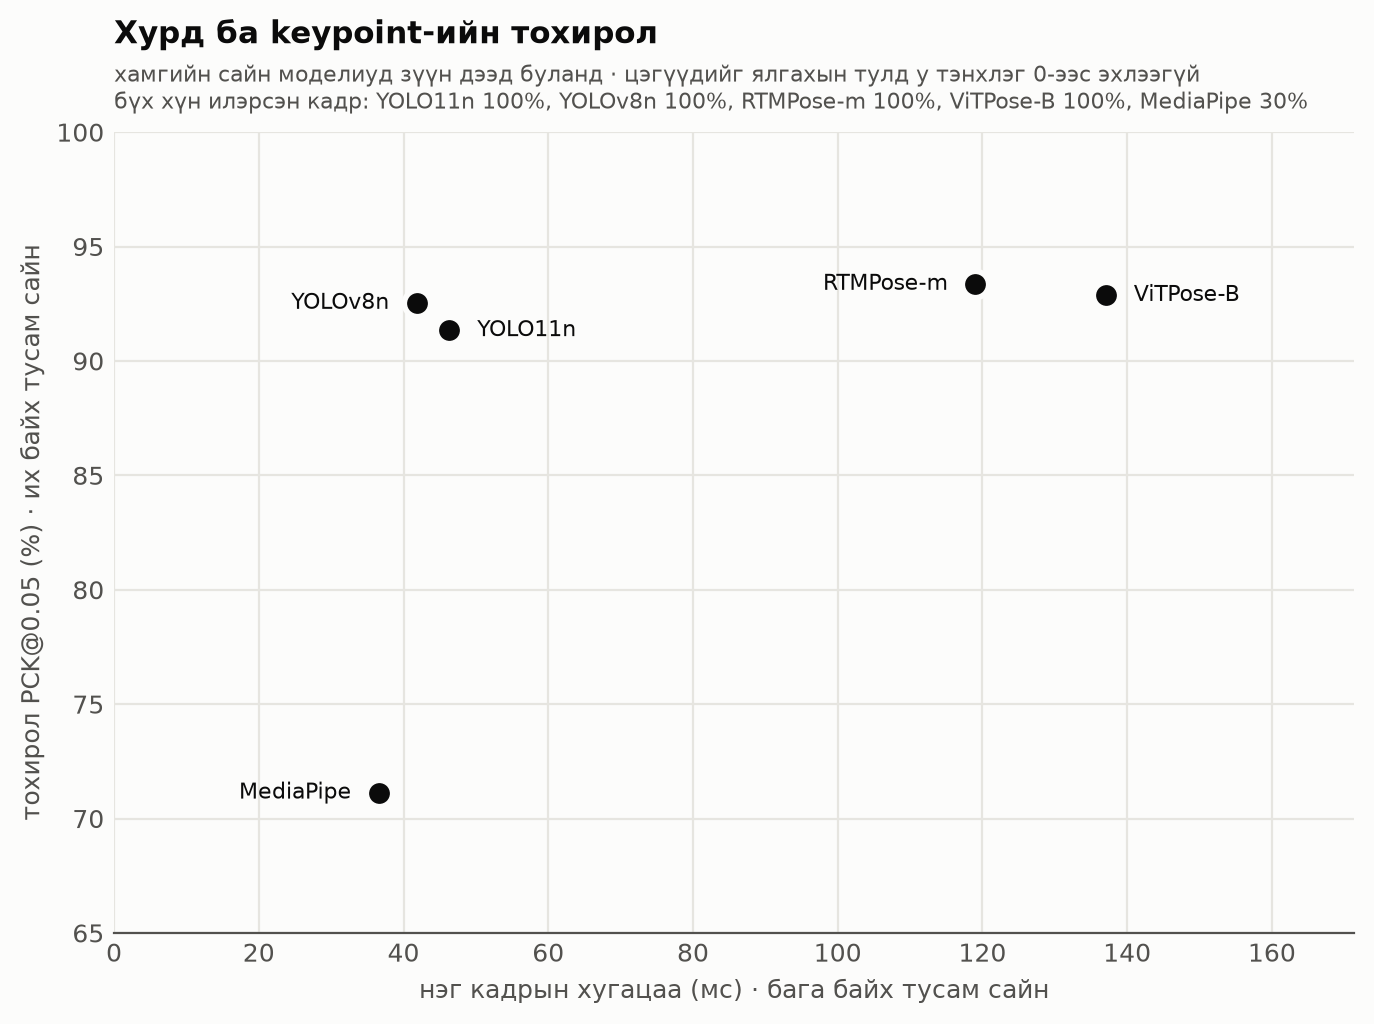
\includegraphics[width=\linewidth]{fig5_tradeoff}
\caption{Хурд ба гол цэгийн тохирлын харьцаа}
\label{fig:fig5_tradeoff}
\end{figure}

\textbf{Нэгдсэн үнэлгээ.} Шалгуур бүрийг хамгийн сайн загварын утгатай харьцуулан (утга ÷ шилдэг утга, бага нь сайн шалгуурт шилдэг утга ÷ утга) 0-1 хооронд хувиргаж, дараах жингээр нэгтгэв: илрүүлэлт 25\%, тохирол 20\%, чичиргээ 20\%, хурд 15\%, худал илрүүлэлт 10\%, мөчдийн тогтвортой байдал 10\%. Анх min-max масштаб ашигласан боловч MediaPipe-ийн хэт муу утгууд бусад дөрвөн загварын хоорондох ялгааг шахаж, MediaPipe-ийг хасахад шилдэг загвар YOLOv8n-ээс RTMPose-m болж өөрчлөгдөж байсан тул харьцааны аргад шилжсэн. Жинлэсэн оноогоор YOLOv8n 91, YOLO11n 90, RTMPose-m 89, ViTPose-B 84, MediaPipe 59 оноо авав (Зураг~\ref{fig:fig6_scorecard}).

\begin{figure}[H]
\centering
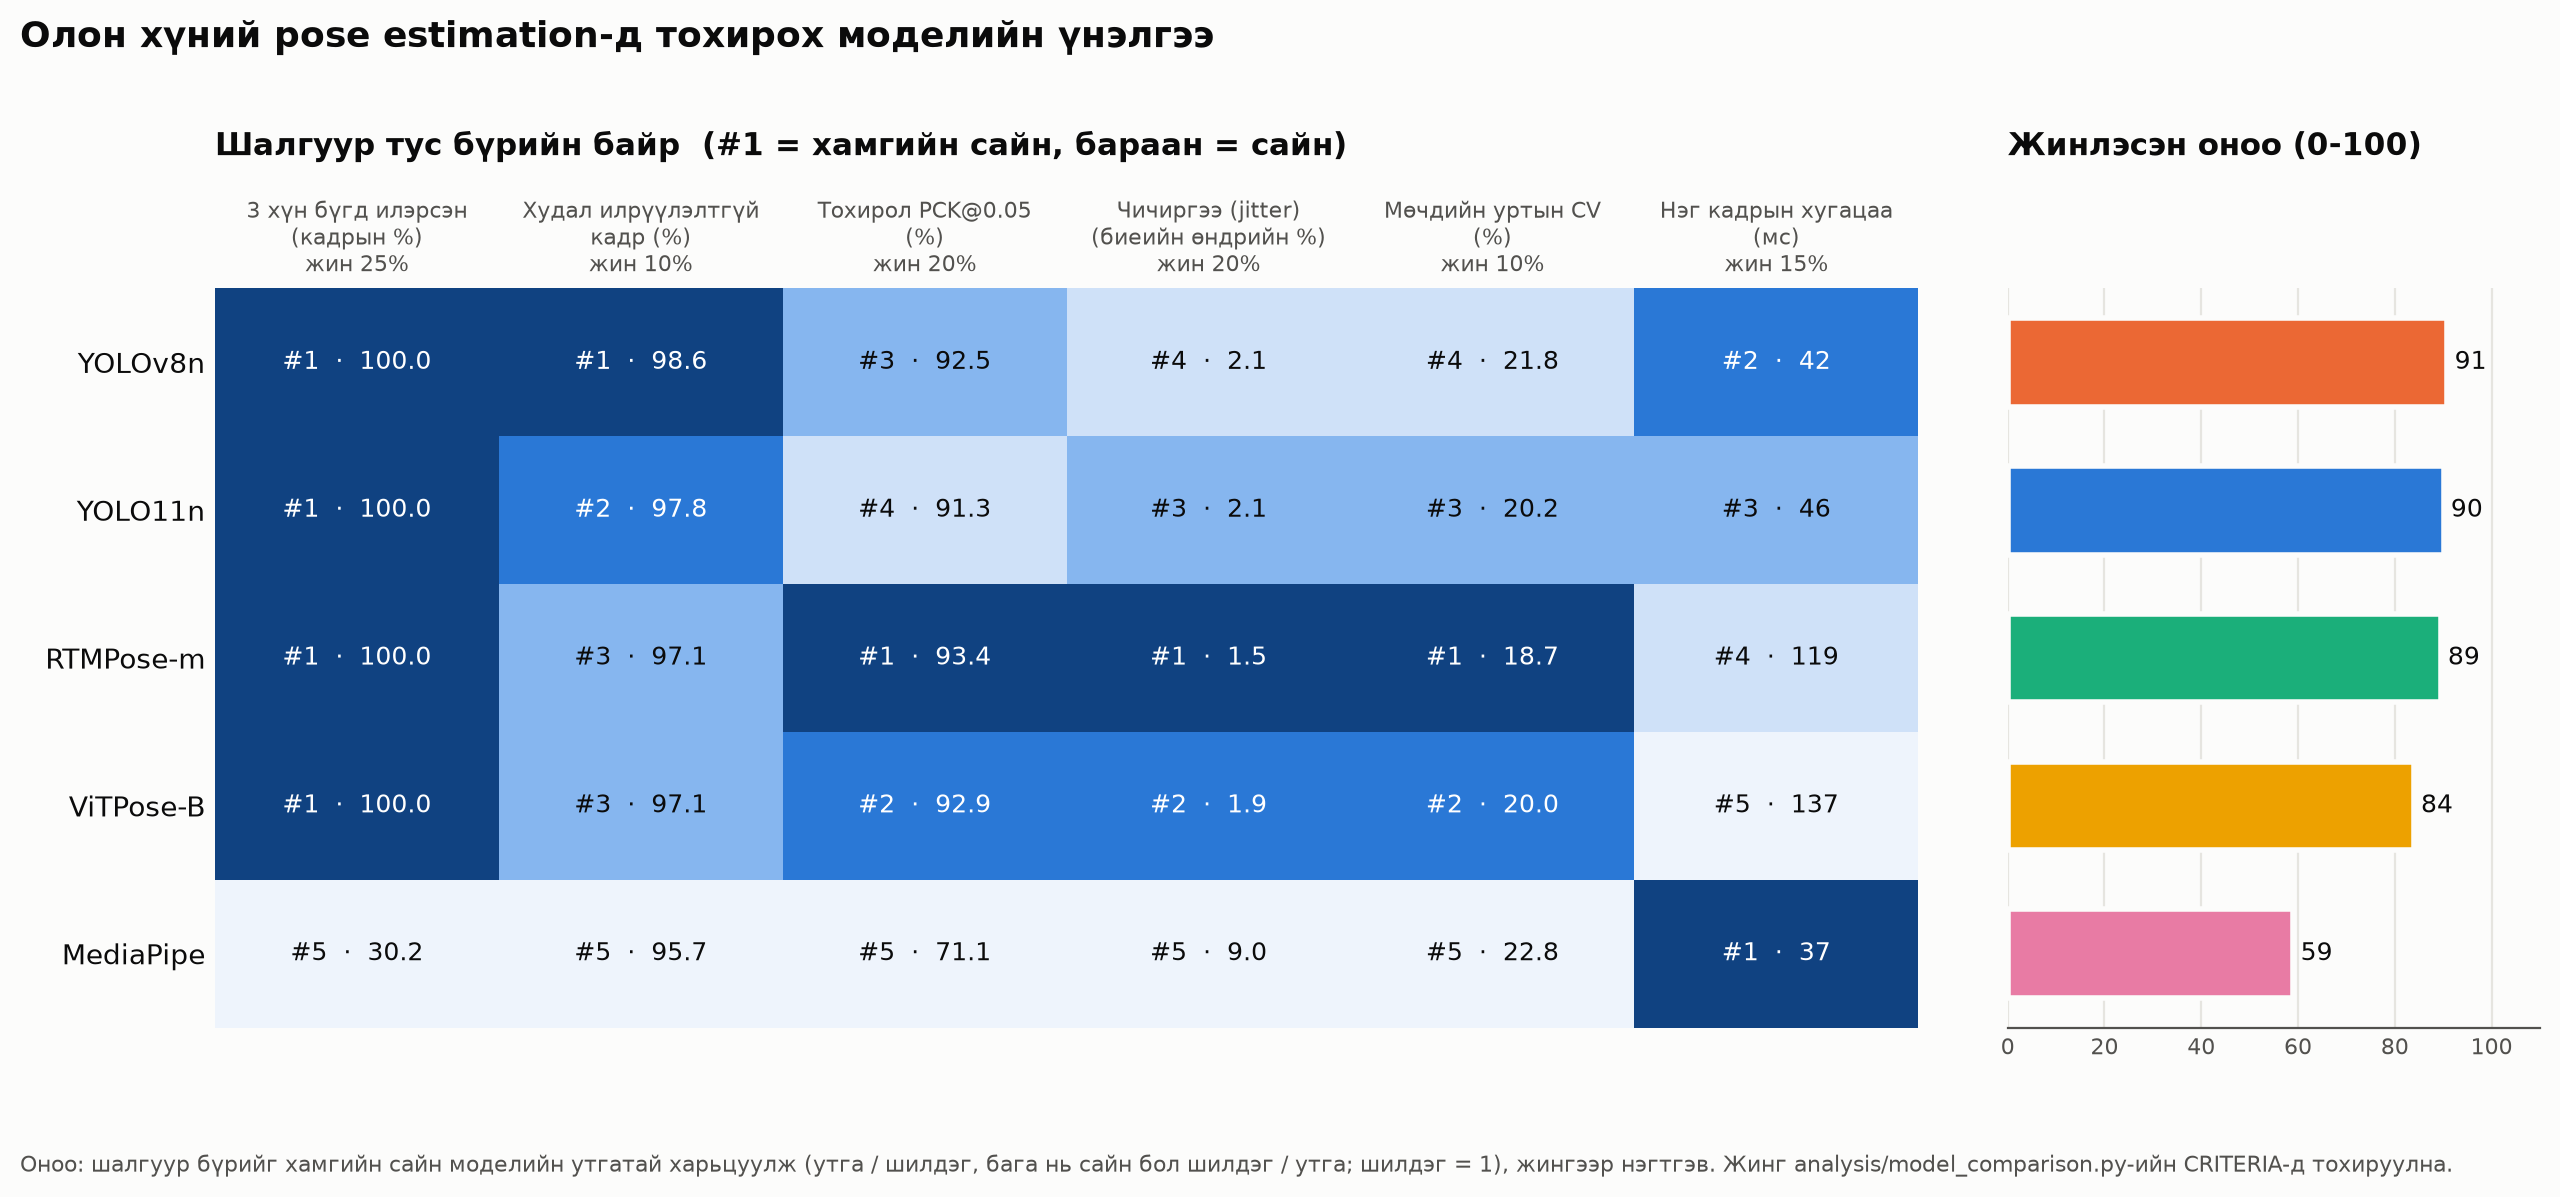
\includegraphics[width=\linewidth]{fig6_scorecard}
\caption{Шалгуур тус бүрийн байр ба жинлэсэн нийт оноо}
\label{fig:fig6_scorecard}
\end{figure}

\textbf{Загвар сонголтын дүгнэлт.} MediaPipe Pose нь нэг хүнд зориулагдсан бөгөөд олон хүнийг тогтвортой илрүүлж чадаагүй тул энэхүү ажилд тохиромжгүй гэж үзэв. Эхний гурван загварын жинлэсэн оноо ердөө 2 онооны зөрүүтэй тул сонголт нь хурд ба гол цэгийн чанарын хоорондын харьцаанаас хамаарна. Энэхүү систем нь шүүгч, дасгалжуулагчдад бичлэгийг дараа нь нарийвчлан шинжлэхэд зориулагдсан бөгөөд тэдний шийдвэр синхрончлолын онооны найдвартай байдлаас шууд хамаарна. Гол цэгийн чичиргээ нь үений өнцгийн хуурамч өөрчлөлт үүсгэж, корреляцид суурилсан оноог бууруулдаг тул хурднаас илүү гол цэгийн чанарыг чухалчлав. Иймд гол цэгийн чанарын бүх үзүүлэлтээр (тохирол 93.4\%, чичиргээ 1.49, мөчдийн уртын хэлбэлзэл 18.7\%), ялангуяа өнцөг тооцоолоход ашиглагдах тохой, бугуй, өвдөг, шагайн цэгүүдийн чичиргээгээр хамгийн сайн үр дүн үзүүлсэн RTMPose-m загварыг сонгов. Жинлэсэн оноогоор YOLOv8n хоёр оноогоор тэргүүлсэн нь хурдны шалгуурт 15\% жин өгсөнтэй холбоотой бөгөөд хурд нь хоёр үе шаттай бүтцийн ачаар (2.6) үр дүнд нөлөөлөхгүй. RTMPose-m-ийн сул тал нь нэг кадрт 119 мс зарцуулж, хүний тоо нэмэгдэхэд удааширдаг явдал боловч хэрэгжүүлэлтийн үндсэн тохиолдол болох хоёр хүнд энэ нь хүлээн зөвшөөрөгдөх хэмжээнд байна.

\textbf{Харьцуулалтын хязгаарлалт.} Ground truth байхгүй тул тохирол нь жинхэнэ нарийвчлал биш, бусад загваруудтай хэр нийцэж буйг л харуулна. Нэг гэр бүлийн загварууд хоорондоо илүү нийцэх хандлагатай бөгөөд YOLOv8n, YOLO11n хоёулаа YOLO гэр бүлийнх, RTMPose-m, ViTPose-B хоёр ижил хүн илрүүлэгч ашигладаг. Шалгууруудын жинг судлаач сонгосон, харьцуулалт нэг бичлэг дээр хийгдсэн, хурдыг браузерийн орчинд хэмжсэн зэргийг үр дүнг тайлбарлахад анхаарах шаардлагатай.

\section{Хүн хуваарилалт}

Бичлэгт хоёр болон түүнээс дээш хүн байх бөгөөд хүмүүс бие биеэ бүрэн халхлахгүй, байраа солихгүй гэж үзнэ. Иймд нарийн мөрдөлтийн (tracking) алгоритм шаардлагагүй бөгөөд кадр бүрт илэрсэн араг ясуудыг гуяны дунд цэгийн x координатаар (гуяны цэгүүд байхгүй үед хүрээний төвөөр) зүүнээс баруун тийш эрэмбэлж, 1, 2, ..., N дугаартай хүнд хуваарилна.

Хүний тоо N-ийг бичлэгийн эхний 2 секундэд хамгийн олон давтагдсан илрүүлэлтийн тоогоор (тэнцүү бол ихийг нь) автоматаар тодорхойлно. Аль нэг кадрт N-ээс олон хүн илэрвэл хүрээний итгэлцэл хамгийн их N илрүүлэлтийг үлдээж, бусдыг нь хасна. N-ээс цөөн хүн илэрвэл илрүүлэлт бүрийг хамгийн сүүлд харагдсан байрлалтай нь хамгийн ойр хүнд шунахай (greedy) аргаар оноож, үлдсэн хүний тухайн кадрын өгөгдлийг дутуу гэж тэмдэглэн 3.4-ийн аргаар нөхнө. Загвар сонголтын бичлэг дээр (856 кадр) 830 кадрт яг гурван хүн, 26 кадрт гурваас олон хүн илэрсэн бөгөөд гурваас цөөн хүн илэрсэн кадр байгаагүй.

\section{Урьдчилсан боловсруулалт}

\textbf{Дутуу ба найдваргүй цэгүүдийг нөхөх.} Итгэлцлийн оноо нь 0.3-аас бага гол цэгүүдийг найдваргүй гэж үзэж, хөрш кадруудын утгаас шугаман интерполяцаар нөхнө. Зөвхөн 1 секундээс богино завсрыг нөхөх бөгөөд үүнээс урт завсар дутуу хэвээр үлдэж, тухайн хугацааны цонхны оноонд оролцохгүй. Загвар сонголтын бичлэг дээр гол цэгийн утгуудын 0.7\%-ийг интерполяцаар нөхсөн.

\textbf{Шуугиан тэгшитгэх.} HPE загварын гаралт кадр бүрт бага зэрэг чичирдэг (jitter) тул координатын цуваа бүрт квадрат олон гишүүнттэй Савицкий-Голейн шүүлтүүр \cite{savitzky1964} хэрэглэнэ. Шүүлтүүрийн цонх ойролцоогоор 0.3 секунд (25 кадр/с давтамжид 9 кадр) бөгөөд хөдөлгөөний хэлбэрийг хадгалахын зэрэгцээ кадр хоорондын санамсаргүй үсрэлтийг бууруулна. Сонгосон RTMPose-m загвар чичиргээ хамгийн багатай байсан ч бугуй, шагайн цэгүүд бусад цэгээс илүү чичирдэг (Зураг~\ref{fig:fig4_keypoint_heatmap}) тул энэ алхам шаардлагатай.

\section{Шинж чанар гаргах}

Кадр бүрт хүн тус бүрийн хувьд дараах найман үений өнцгийг тооцоолно. Өнцөг бүрийг 2.4-т өгсөн томьёогоор гурван гол цэгээс тооцоолно (дугаар нь COCO форматын индекс). Тооцоололд арккосинустай тэнцүү \(\theta = \operatorname{atan2}(|u \times v|, \; u \cdot v)\) хэлбэрийг (\(u = a - b, \; v = c - b\)) ашигласан нь 0° болон 180°-ийн орчимд тоон алдаа багатай.

\begin{table}[H]
\centering
\caption{Үений өнцгийг тооцоолох гол цэгүүд}
\label{tab:joints}
\small
\begin{tabular}{|>{\raggedright\arraybackslash}p{0.234\linewidth}|>{\raggedright\arraybackslash}p{0.260\linewidth}|>{\raggedright\arraybackslash}p{0.372\linewidth}|}
\hline
\textbf{Үе} & \textbf{Гол цэгүүд (a, b, c)} & \textbf{Биеийн хэсэг} \\ \hline
Зүүн тохой & мөр 5, тохой 7, бугуй 9 & Гар \\ \hline
Баруун тохой & мөр 6, тохой 8, бугуй 10 & Гар \\ \hline
Зүүн мөр & гуя 11, мөр 5, тохой 7 & Гар \\ \hline
Баруун мөр & гуя 12, мөр 6, тохой 8 & Гар \\ \hline
Зүүн гуя & мөр 5, гуя 11, өвдөг 13 & Их бие \\ \hline
Баруун гуя & мөр 6, гуя 12, өвдөг 14 & Их бие \\ \hline
Зүүн өвдөг & гуя 11, өвдөг 13, шагай 15 & Хөл \\ \hline
Баруун өвдөг & гуя 12, өвдөг 14, шагай 16 & Хөл \\ \hline
\end{tabular}
\end{table}

Гуяны өнцөг нь мөр, гуя, өвдөг гэсэн цэгүүдээр тодорхойлогддог тул хөл болон их биеийн аль алинд хамаарах боловч биеийн хэсгүүдийн жин давхар тоологдохгүйн тулд их биед хамааруулсан. Ингээд гар нь хоёр тохой ба хоёр мөр (4 үе), хөл нь хоёр өвдөг (2 үе), их бие нь хоёр гуя (2 үе) болно.

\textbf{Биеийн хэсгийн жин.} Синхрончлолын оноонд бүх үеийг тэнцүү тооцохын оронд биеийн хэсгээр (гар, хөл, их бие) хувааж жигнэнэ. Биеийн хэсгийн жинг тухайн хэсгийн үеүдэд тэнцүү хуваарилж, бүх үеийн жингийн нийлбэр 1 болохоор хэвийн болгон үе бүрийн жин \(\alpha_k\)-г гаргана. Энэхүү ажилд гарт 50\%, хөлд 25\%, их биед 25\% жин өгсөн бөгөөд ингэхэд тохой, мөр, өвдөг, гуя тус бүр 12.5\% жинтэй болно. Жингийн утгыг судлаач тогтоосон бөгөөд спортын төрлөөс хамааран өөрчлөх боломжтой.

\section{Синхрончлолын алгоритм}

Синхрончлолыг гурван бүрэлдэхүүн хэсгээр үнэлж, тэдгээрийг нэгтгэн нэг оноо гаргана. Анх төлөвлөсөн аргыг (хувилбар 1) хэрэгжүүлж туршсаны дараа цонхны хэлбэр, үений жин, толин тусгал горимын сонголтыг сайжруулсан бөгөөд энэ хэсэгт эцсийн буюу сайжруулсан хувилбарыг (хувилбар 2) тайлбарлав. Алгоритмын бүх параметрийг секундээр тодорхойлж, видеоны кадрын давтамж f-ээр кадр руу хөрвүүлдэг тул өөр давтамжтай бичлэг дээр ижил утгатай ажиллана.

\textbf{Гулсах цонх.} Кадр бүрт тухайн кадрыг голдоо агуулсан W = 2 секунд урттай нэг цонх (\(t - W/2 \ldots t + W/2\)) үүсгэнэ. Бичлэгийн эхлэл, төгсгөлд цонх видеоноос гарах тул түүнийг видеоны дотор шилжүүлж, урт нь W хэвээр үлдэнэ. Ингэснээр бүрэлдэхүүн бүрийн оноо кадр бүрт тодорхойлогдож, видеог тоглуулахад тухайн мөчийн оноог цагийн тэмдгээр шууд харуулах боломжтой болно.

\textbf{Байрлалын ижил төстэй байдал.} Цонхонд хоёр хүний харгалзах үений өнцгийн абсолют зөрүүний дунджийг үе бүрээр тооцоолж, үений жингээр нэгтгэнэ:

\begin{equation}
S_{pose} = 1 - \sum_{k=1}^{K} \alpha_k \frac{\bar{d}_k}{180^{\circ}}, \qquad \bar{d}_k = \frac{1}{|T_k|} \sum_{t \in T_k} \left| \theta^{A}_{k}(t) - \theta^{B}_{k}(t) \right|
\end{equation}

Энд \(T_k\) нь цонхны k үеийн хоёр хүнд хоёуланд нь утгатай кадрууд бөгөөд өгөгдөлгүй үеийг хасаж, үлдсэн үеүдийн жинг нийлбэр нь 1 болохоор дахин хэвийн болгоно. Цонхны утгуудын тал хувиас бага нь байгаа бол тухайн цонхонд оноо өгөхгүй.

\textbf{Хөдөлгөөний уялдаа.} Цонхонд үе тус бүрийн өнцгийн цуваануудын Пирсоны корреляц \(r_k\)-г тооцоолж, үений жингээр нэгтгэнэ:

\begin{equation}
S_{corr} = \frac{1}{2} \left( \sum_{k} \alpha_k r_k + 1 \right)
\end{equation}

Хоёр хүнд хоёуланд нь өнцгийн стандарт хазайлт 3°-аас бага, өөрөөр хэлбэл бараг хөдөлгөөнгүй үеийн корреляц нь шуугианаас хамаардаг тул түүнийг \(S_{corr}\) болон хоцрогдлын тооцооллоос хасна. Нэг хүн тухайн үеэ хөдөлгөж, нөгөө нь хөдөлгөөгүй бол \(r_k = 0\) гэж үзнэ. Цонхонд аль ч үе хөдлөөгүй, өөрөөр хэлбэл хоёр хүн хоёулаа байрлалаа барьж зогссон бол корреляц болон хоцрогдол тодорхойгүй тул оноог зөвхөн \(S_{pose}\)-оор гаргана.

\textbf{Цагийн хоцрогдол.} Хоёр хүний өнцгийн өөрчлөлтийн хурдны (кадр хоорондын ялгавар) цуваанд хэвийн болгосон хөндлөн корреляцыг хэрэглэж, хөдөлж буй үеүдийн \(\rho(\tau)\)-ийн дундаж хамгийн их байх \(\tau^{*}\) шилжилтийг \(|\tau| \le \tau_{max}\) мужид олно. Тэнцүү утгатай бол хамгийн бага \(|\tau|\)-г сонгоно. Хоцрогдлын оноог дараах байдлаар тооцоолно:

\begin{equation}
S_{lag} = \begin{cases} \max\left(0, \; 1 - \dfrac{|\tau^{*}|}{\tau_{max}}\right), & \rho_{max} \ge \rho_{min} \\ 0, & \rho_{max} < \rho_{min} \end{cases}
\end{equation}

Хоёр хүн огт өөр хөдөлгөөн хийсэн үед хөндлөн корреляц санамсаргүй нэг шилжилтийг «хамгийн сайн» гэж сонгодог тул \(\rho_{min}\) босгоор олдсон хоцрогдолд итгэх эсэхийг шийднэ. Хамгийн их хайх хоцрогдол \(\tau_{max} = 1.5\) секунд бөгөөд энэ нь туршсан хамгийн их хоцрогдлоос (1 секунд) их байх ёстой. Босгын утгыг загвар сонголтын бичлэг дээр гол цэгийн түвшний хяналттай хосоор тохируулсан. Хамт хөдөлж буй хүмүүсийн цонхнуудын \(\rho_{max}\)-ийн медиан ойролцоогоор 0.42, өөр хөдөлгөөнтэй хосынх 0.13, яг ижил хуулбарынх 1.0 байв. Иймд төлөвлөж байсан 0.5 босго бодит синхрон хөдөлгөөнийг ч үгүйсгэж байсан тул хоёр бүлгийг ялгах \(\rho_{min} = 0.3\) утгыг сонгов. Энэ босгын орчимд \(S_{lag}\) огцом өөрчлөгддөг сул талтай болох нь хожим илэрсэн бөгөөд үүнийг 4.4-т тайлбарлав.

\textbf{Нэгдсэн оноо.} Гурван бүрэлдэхүүнийг жигнэсэн нийлбэрээр нэгтгэж, 0-100 хуваарьт шилжүүлнэ:

\begin{equation}
S = 100 \cdot \left( w_1 S_{pose} + w_2 S_{corr} + w_3 S_{lag} \right), \qquad w_1 + w_2 + w_3 = 1
\end{equation}

Бүрэлдэхүүнүүд \(w_1 = w_2 = w_3 = 1/3\) тэнцүү жинтэй бөгөөд аль нэг бүрэлдэхүүн тодорхойгүй үед (жишээлбэл, хөдөлгөөнгүй цонх) үлдсэн бүрэлдэхүүнүүдийн жинг дахин хэвийн болгоно. Хосын бүх бичлэгийн оноо нь цонхнуудын онооны дундаж, бүх бичлэгийн хоцрогдол нь бүтэн цувааны хөндлөн корреляцаар олдсон \(\tau^{*}\) байна. Биеийн хэсэг бүрийн (гар, хөл, их бие) оноог зөвхөн тухайн хэсгийн үеүдийг тэнцүү жинтэйгээр ашиглан ижил аргаар тооцоолж, аль хэсэгт синхрончлол алдагдаж байгааг тодорхойлно.

\textbf{Хоёр горимт харьцуулалт.} Бүжгийн найруулга ердийн эсвэл толин тусгал байхаас хамааран харьцуулах арга өөр болно (2.4). Иймд цонх бүрт ердийн болон толин тусгал (Б хүний зүүн, баруун үеүдийг сольсон) гэсэн хоёр горимоор оноо тооцоолно. Толин тусгал горимын оноо ердийн горимынхоос дор хаяж 5 оноогоор их байвал л толин тусгал горимыг сонгож, бусад тохиолдолд ердийн горимыг хэрэглэнэ. Энэ нь хоёр горимын оноо ойролцоо байх үед горим цонх бүрээр солигдож анивчихаас сэргийлэхээс гадна нэг бүжигчин санамсаргүй буруу гараа хөдөлгөхөд систем үүнийг толин тусгал гэж үзэж алдааг нуух эрсдэлийг бууруулна. Найруулгын горим урьдчилан мэдэгдэж байгаа тохиолдолд хэрэглэгч горимыг тогтмол сонгох боломжтой.

\textbf{Олон хүний синхрончлол.} Дээрх тооцоолол нь хоёр хүний хоорондох синхрончлолыг үнэлдэг бөгөөд энэ нь аргын үндсэн бөгөөд хамгийн оновчтой тохиолдол юм. Бичлэгт N хүн байх үед бүлэгт гол хүн (дасгалжуулагч, ахлагч) байхгүй, бүх хүн тэгш эрхтэй гэж үзэж, хүн бүрийг бусад бүх хүнтэй хос хосоор нь харьцуулна. Хосын тоо \(N(N-1)/2\) бөгөөд гурван хүнд 3, дөрвөн хүнд 6 хос болно. i ба j хүний хоорондох синхрончлолын оноог \(S_{ij}\) гэвэл бүлгийн нийт оноог бүх хосын онооны дунджаар, i-р хүний оноог түүний оролцсон хосуудын онооны дунджаар тооцоолно:

\begin{equation}
S_{group} = \frac{2}{N(N-1)} \sum_{i<j} S_{ij}, \qquad S_i = \frac{1}{N-1} \sum_{j \ne i} S_{ij}
\end{equation}

Хүн тус бүрийн оноо \(S_i\) нь бүлгээсээ хамгийн их зөрж буй хүнийг тодорхойлох боломж олгоно. Хоёр горимт харьцуулалт болон хоцрогдлын тооцоолол хос бүрт тусдаа хийгдэнэ. Хосын тоо хүний тоотой квадратаар өсдөг боловч тооцоолол нь өнцгийн цуваан дээр хийгдэх тул HPE загварын тооцооллоос хамаагүй бага бөгөөд гурван хүнтэй 856 кадрын бичлэгийн синхрончлолыг бүхэлд нь хэдхэн секундэд тооцоолж байна.

\textbf{Синхрончлол алдагдсан мөчүүд.} Бүлгийн нэг тоон оноо нь хэзээ, хэн, биеийн аль хэсгээрээ зөрснийг харуулдаггүй тул хос бүрт синхрончлол алдагдсан хугацааны хэсгүүдийг (мөчүүдийг) тусад нь илрүүлнэ. Цонхыг дараах нөхцлийн аль нэг биелэхэд «зөрсөн» гэж тэмдэглэнэ. Үүнд:

\begin{itemize}
\item
  Цонхны \(S_{corr}\) нь тухайн хосын бүх бичлэгийн медианаас 0.15-аар, эсвэл \(S_{pose}\) нь медианаас 0.06-аар бага байх. Хос бүрийг өөрийнх нь ердийн түвшинтэй харьцуулдаг тул байнга бага зэрэг зөрдөг хос нэг урт мөч болж харагдахгүй.
\item
  Бүх бие найдвартай хоцорсон байх: \(|\tau^{*}| \ge 0.2\) секунд ба \(\rho_{max} \ge \rho_{min}\).
\item
  Аль нэг мөч (зүүн, баруун гар нь тохой ба мөр, зүүн, баруун хөл нь гуя ба өвдөг) хоцорсон байх. Хоёр дахь хүний тухайн мөчийг τ-гаар шилжүүлэхэд өнцгийн дундаж зөрүү \(D(\tau)\) мэдэгдэхүйц багасвал, өөрөөр хэлбэл \(D(0) - \min D(\tau) \ge 3^{\circ}\) ба \(D(0)\)-ийн 20\%-иас их, мөн \(0.2 \le |\tau| < \tau_{max}\) секунд байвал мөчийг хоцорсон гэж үзнэ. Энэ нөхцөл нь нэг гар хоцорч, бусад хэсэг нь зэрэг хөдөлж буй, бүх биеийн оноонд дундажлагдан алга болдог тохиолдлыг илрүүлнэ.
\end{itemize}

Нийт 1 секундээс урт хугацааг хамарсан зөрсөн цонхнууд (0.5 секундээс богино завсрыг нэгтгэж) нэг мөч болно. Мөч бүрт хоцорсон мөч болон хоцрогдлыг, мөн хоцорсон мөчийн үе бүрийн хувьд тухайн шилжилт зөрүүг 2°-аас их багасгасан эсэхийг (хоцорсон үе), эсвэл өнцгийн зөрүү нь бичлэгийн ердийн зөрүүнээс 15°-аас их байгаа эсэхийг (өөр хөдөлгөөнтэй үе) тодорхойлж харуулна. «Хоцорсон» гэж тооцох доод хоцрогдол нь анхдагчаар 0.2 секунд бөгөөд хэрэглэгч үүнийг 0.12--1.0 секундийн хооронд өөрчилж болох ч энэ нь зөвхөн жагсаах мөчүүдэд нөлөөлж, оноог өөрчлөхгүй. 0.12 секундээс бага утгад синхрон хосын цонхнуудад ч хэмжигддэг 0.04--0.16 секундийн хоцрогдол мөч болж тоологдон, бичлэгийн бараг тал нь зөрсөн гэж тэмдэглэгдэж байсан тул доод хязгаарыг 0.12 секунд болгосон.

Алгоритмын эхний (хувилбар 1) болон сайжруулсан (хувилбар 2) хувилбарын ялгааг доорх хүснэгтэд нэгтгэв.

\begin{table}[H]
\centering
\caption{Синхрончлолын алгоритмын хувилбаруудын ялгаа}
\label{tab:versions}
\small
\begin{tabular}{|>{\raggedright\arraybackslash}p{0.200\linewidth}|>{\raggedright\arraybackslash}p{0.320\linewidth}|>{\raggedright\arraybackslash}p{0.360\linewidth}|}
\hline
\textbf{Шинж} & \textbf{Хувилбар 1} & \textbf{Хувилбар 2} \\ \hline
Цонх & 3 секунд, 0.5 секунд тутамд & 2 секунд, кадр бүрт, кадр голдоо \\ \hline
Үений жин & Бүх үе тэнцүү & Биеийн хэсгийн жингээс \(\alpha_k\) (гар 50\%, хөл 25\%, их бие 25\%) \\ \hline
Биеийн хэсэг & Хөл = гуя ба өвдөг, их бие = гуя & Хөл = өвдөг, их бие = гуя (давхардалгүй) \\ \hline
Толин тусгал & Өндөр оноотой горимыг сонгоно & 5 оноогоор илүү бол л толин тусгал \\ \hline
Гаралт & Цонх бүрийн CSV & Нэмээд кадр бүрийн CSV (цагийн тэмдэгтэй) \\ \hline
\end{tabular}
\end{table}

Хувилбар 2-ын ерөнхий бүтцийг доорх хуурмаг кодоор (pseudocode) харуулав.

\begin{lstlisting}[language=Python, caption={Синхрончлолын алгоритмын хуурмаг код (хувилбар 2)}, label={lst:sync}, frame=single, columns=fullflexible, keepspaces=true]
def group_sync(frames, fps, W=2.0, tau_max=1.5, rho_min=0.3,
               w=(1/3, 1/3, 1/3), part_weights=GENERAL, margin=5):
    N = most_common_count(frames, first_seconds=2)
    people = assign_left_to_right(frames, N)           # гуяны x-ээр 1..N
    people = [preprocess(p) for p in people]           # нөхөх, тэгшитгэх
    angles = [joint_angles(p) for p in people]         # хүн бүрт (8, T)
    alpha = joint_weights(part_weights)                # alpha_k, нийлбэр 1

    S = zeros((N, N))
    for i, j in combinations(range(N), 2):             # хос бүр
        frame_scores = []
        for t in range(len(frames)):                   # кадр бүрт нэг цонх
            win = centred_window(t, W * fps)
            s_n = window_score(angles[i], angles[j], win, alpha)
            s_m = window_score(angles[i], mirror(angles[j]), win, alpha)
            frame_scores.append(s_m if s_m >= s_n + margin else s_n)
        S[i, j] = S[j, i] = mean(frame_scores)
    group = mean([S[i, j] for i, j in combinations(range(N), 2)])
    per_person = [sum(S[i]) / (N - 1) for i in range(N)]
    return group, per_person

def window_score(a, b, win, alpha):
    s_pose = 1 - weighted_mean(abs(a[:, win] - b[:, win]), alpha) / 180
    moving = [k for k in range(8) if std(a[k, win]) >= 3 or std(b[k, win]) >= 3]
    if not moving:
        return 100 * s_pose                            # хоёулаа хөдөлгөөнгүй
    s_corr = (weighted_mean(pearson(a[k, win], b[k, win]) for k in moving) + 1) / 2
    tau, rho_max = normalized_cross_corr(diff(a), diff(b), win, moving, tau_max)
    s_lag = max(0, 1 - abs(tau) / tau_max) if rho_max >= rho_min else 0
    return 100 * (w[0] * s_pose + w[1] * s_corr + w[2] * s_lag)
\end{lstlisting}

\section{Хэрэгжүүлэлтийн орчин}

Системийг 2.6-д тайлбарласан технологиудаар хэрэгжүүлсэн. Хэрэглэгч видеог аль орчинд боловсруулахаа хуудсан дээрх «Process videos on: This browser / Server» сонголтоор шийднэ.

\textbf{Вэб хөтчийн горим.} RTMPose-m загвар болон түүний YOLO11n хүн илрүүлэгчийг ONNX Runtime Web сангаар WebGPU backend дээр (боломжгүй үед WASM) ажиллуулна. Видеог кадр бүрээр уншиж, загварын гаралтаас араг яс зурагдсан видео, үр дүнгийн файлуудыг үүсгэнэ.

\textbf{Серверийн горим.} Вэб аппликейшн нээлттэй байгаа видео файлыг Python серверт илгээж, сервер ижил ONNX файлуудыг ONNX Runtime-ээр CUDA (NVIDIA GPU) дээр, боломжгүй үед CPU дээр ажиллуулна. Серверийн боловсруулалт нь хөтчийнхтэй ижил алхмуудаас бүрдэнэ. Үүнд: хүн илрүүлэгчийн оролтыг 640×640 хэмжээнд харьцааг нь хадгалан багасгаж саарал (114) өнгөөр дүүргэх, зөвхөн хүний ангиллыг авч давхацсан илрүүлэлтүүдийг IoU 0.7 босготой NMS-ээр шүүх, хүрээг 1.25 дахин томруулж загварын харьцаанд тааруулан 192×256 хэмжээнд тайрах, ImageNet-ийн дундаж, стандарт хазайлтаар хэвийн болгох, SimCC гаралтаас x, y тэнхлэг тус бүрийн хамгийн их утгаар гол цэгийг тодорхойлох. Видеог OpenCV-ээр кадр бүрээр, алгасахгүйгээр уншиж, хөтчийн хадгалдагтай яг ижил бүтэцтэй гол цэгийн JSON буцаана. Сервер зөвхөн гол цэгийг тодорхойлох бөгөөд синхрончлол, статистик, үр дүн хадгалах ажлыг вэб аппликейшн хөтчийн горимтой адил гүйцэтгэдэг тул хоёр горимын үр дүн шууд харьцуулагдана. Араг яс зурагдсан видеог буцаасан гол цэгүүдээс хөтөч дээр зурна. Серверийн API-ийг доорх хүснэгтэд үзүүлэв.

\begin{table}[H]
\centering
\caption{HPE серверийн API}
\label{tab:api}
\small
\begin{tabular}{|>{\raggedright\arraybackslash}p{0.330\linewidth}|>{\raggedright\arraybackslash}p{0.560\linewidth}|}
\hline
\textbf{Хүсэлт} & \textbf{Үүрэг} \\ \hline
\texttt{GET /health} & Серверийн төлөв, загварууд болон тэдгээрийн ажиллах төхөөрөмж \\ \hline
\texttt{POST /jobs} & Видео, загварын нэр, итгэлцлийн босго, кадрын давтамж, кадрын тоог хүлээн авч ажлын дугаар буцаана \\ \hline
\texttt{GET /jobs/\{id\}} & Ажлын төлөв (дараалалд, ажиллаж байна, дууссан, алдаа) ба явцын хувь \\ \hline
\texttt{GET /jobs/\{id\}/keypoints} & Кадр бүрийн гол цэгүүд (хөтчийн форматаар) \\ \hline
\texttt{DELETE /jobs/\{id\}} & Ажлыг цуцалж устгах \\ \hline
\end{tabular}
\end{table}

GPU нэгэн зэрэг олон ажлыг гүйцэтгэхэд удаашрах тул сервер ажлуудыг дараалалд оруулж нэг нэгээр нь гүйцэтгэх бөгөөд илгээсэн видеог ажил дуусмагц устгана. Үр дүнгийн JSON файлд тухайн ажиллуулалт аль горимд хийгдсэн (\texttt{backend}), серверийн горимд видео илгээх болон серверийн боловсруулалтын хугацааг хадгалдаг тул хоёр горимын хурд, үр дүнг дараа нь харьцуулах боломжтой.

\textbf{Үр дүнгийн файлууд.} Ажиллуулалт бүр гол цэгийн JSON, CSV, кадр бүрийн хүний тоо, загварын харьцуулалтын хэмжүүрүүд, араг яс зурагдсан MP4 видео болон синхрончлолын үр дүнг үүсгэнэ. Синхрончлолын үр дүнд бүх бичлэгийн дүн (JSON), хос бүрийн цонхны оноо (CSV), кадр бүрийн оноо (CSV; цагийн тэмдэг, бүлгийн оноо, хүн тус бүрийн оноо, хос бүрийн оноо, хоцрогдол мс-ээр, горим, гар, хөл, их биеийн оноо) болон кадр бүрийн үений өнцөг (CSV) багтана. Ижил бичлэгийг дахин боловсруулахад өмнөх файлуудыг дарж бичихгүй, шинэ дугаартай файл үүсгэнэ.

\textbf{Туршилтын хэрэгслүүд.} Синхрончлолын алгоритм нь вэб хөтөч болон Node.js орчинд хоёуланд ажиллахаар бичигдсэн тул хадгалсан гол цэгийн файлууд дээр алгоритмыг тушаалын мөрөөс параметрүүдийг нь өөрчлөн дахин ажиллуулах боломжтой. Туршилтын үр дүнгийн шинжилгээ болон тайлангийн графикуудыг Python хэл дээр Pandas, NumPy, Matplotlib сангуудаар гаргана.
